% ============================================================
%  Sprawozdanie: Badanie polaryzacji światła (POLAR)
%  Fotonika – laboratorium, ZUT Szczecin
% ============================================================
\documentclass[a4paper,12pt]{article}

\usepackage[utf8]{inputenc}
\usepackage[T1]{fontenc}
\usepackage{lmodern}
\usepackage[polish]{babel}
\usepackage{geometry}
\geometry{a4paper, top=2.2cm, bottom=2.2cm, left=2.5cm, right=2.5cm}

\usepackage{amsmath,amssymb}
\usepackage{booktabs}
\usepackage{graphicx}
\usepackage{float}
\usepackage{caption}
\usepackage{multirow}
\usepackage{array}
\usepackage{xcolor}
\usepackage{hyperref}
\usepackage{siunitx}
\sisetup{output-decimal-marker={,}, locale=DE}
\usepackage{parskip}
\setlength{\parskip}{4pt}

\graphicspath{{../}}

\title{}
\date{}

\begin{document}

% ============================================================
%  TABELA NAGŁÓWKOWA (punkty 1–3)
% ============================================================
\begin{table}[H]
\centering
\small
\renewcommand{\arraystretch}{1.3}
\resizebox{\textwidth}{!}{%
\begin{tabular}{|*{12}{c|}}
\hline
\multicolumn{12}{|c|}{\textbf{Zachodniopomorski Uniwersytet Technologiczny w Szczecinie}} \\
\hline
\multicolumn{2}{|c|}{Przedmiot:} & \multicolumn{10}{c|}{Fotonika} \\
\hline
\multicolumn{2}{|c|}{Prowadzący:} & \multicolumn{10}{c|}{Mgr. Inż. Eliza Miśkiewicz} \\
\hline
\multicolumn{12}{|c|}{\textbf{SPRAWOZDANIE Z WYKONANEGO ĆWICZENIA}} \\
\hline
\multicolumn{2}{|c|}{Nr ćw.: 8} & 02 & \multicolumn{2}{c|}{Temat:} & \multicolumn{7}{c|}{POLARYZACJA (POLAR)} \\
\hline
Zespół lab.: & 5 & Grupa: & L1 & Studia: & S2 & Kierunek: & TI & Rok: & 2025/2026 & Data: & 27.04.2026 \\
\hline
\multicolumn{3}{|c|}{Skład zespołu wg. obecności podczas ćwiczenia:} & \multicolumn{9}{c|}{1. Kamil Suchy} \\
\hline
\multicolumn{2}{|c|}{Ocena:} & \multicolumn{10}{c|}{} \\
\hline
\end{tabular}%
}
\end{table}

% ============================================================
\section*{Cel ćwiczenia}
% ============================================================

Celem ćwiczenia było poznanie zjawiska polaryzacji światła, doświadczalne wyznaczenie
kąta Brewstera dla płytki kwarcowej, obliczenie jej współczynnika załamania $n$ oraz
zbadanie skuteczności stosu polaryzacyjnego (15 płytek szklanych) jako polaryzatora
liniowego.

% ============================================================
\section*{Wstęp teoretyczny}
% ============================================================

Światło jako poprzeczna fala elektromagnetyczna może być spolaryzowane -- oznacza to,
że wektor pola elektrycznego $\mathbf{E}$ drga w uporządkowany sposób. Wyróżnia się
polaryzację liniową, kołową i eliptyczną. W świetle naturalnym (niespolaryzowanym)
kierunek $\mathbf{E}$ zmienia się chaotycznie.

\textbf{Prawo Malusa} wiąże natężenie światła przechodzącego przez analizator z kątem
$\varphi$ między osią polaryzacji a osią transmisji analizatora:
\[
I = I_0 \cos^2\varphi .
\]
Przy $\varphi = 90^\circ$ natężenie spada do zera -- wiązka zostaje wygaszona.

\textbf{Polaryzacja przez odbicie.} Gdy światło pada na granicę dielektryka, wiązka
odbita ulega częściowej polaryzacji. Przy pewnym szczególnym kącie padania $\theta_B$,
zwanym kątem Brewstera, wiązka odbita jest całkowicie spolaryzowana liniowo (zawiera
(tylko składową s, prostopadłą do płaszczyzny padania). Kąt Brewstera spełnia zależność
wynikającą z prawa Snella i warunku $\theta_i + \theta_t = 90^\circ$:
\[
n = \tan\theta_B .
\]
Pomiar $\theta_B$ umożliwia zatem wyznaczenie współczynnika załamania dielektryka.

\textbf{Stos polaryzacyjny} składa się z wielu płytek ustawionych pod kątem Brewstera.
Przy każdym odbiciu usuwana jest część składowej s z wiązki przechodzącej, podczas gdy
składowa p przechodzi bez strat ($r_p = 0$). Dla $N$ płytek o współczynniku odbicia $R_s$
dla składowej s, stopień polaryzacji wiązki przechodzącej rośnie z liczbą odbić:
\[
P = \frac{1 - (1-R_s)^{2N}}{1 + (1-R_s)^{2N}} .
\]
Dla $N=15$ płytek szklanych oczekuje się $P > 0{,}98$. Doświadczalnie stopień polaryzacji
wyznacza się z pomiarów $I_{\max}$ i $I_{\min}$ za obracanym analizatorem:
\[
P = \frac{I_{\max} - I_{\min}}{I_{\max} + I_{\min}} .
\]

% ============================================================
\section*{Schematy układów pomiarowych}
% ============================================================

\begin{figure}[H]
\centering
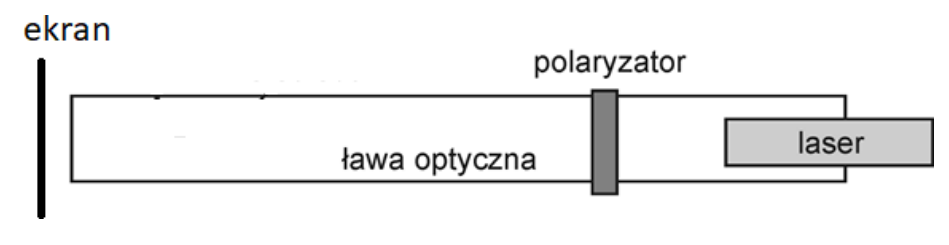
\includegraphics[width=0.85\textwidth]{Rys1.png}
\caption{Układ do analizy stanu polaryzacji światła generowanego przez laser
(Laser He-Ne, P -- polaryzator obrotowy, E -- ekran/detektor).}
\end{figure}

\begin{figure}[H]
\centering
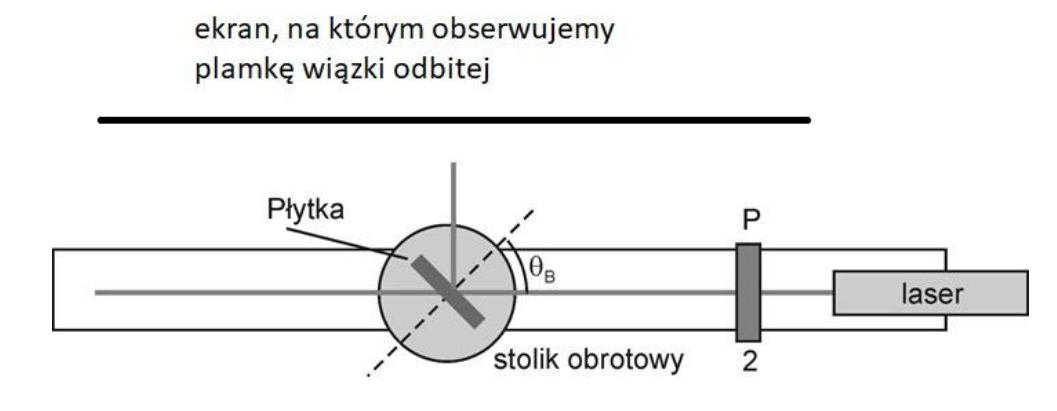
\includegraphics[width=0.85\textwidth]{Rys2.png}
\caption{Układ do wyznaczenia kąta Brewstera. P -- polaryzator z poziomą osią
transmisji, płytka kwarcowa na stoliku obrotowym, E -- ekran, FD -- fotodetektor.}
\end{figure}

% ============================================================
\section*{Spis przyrządów pomiarowych}
% ============================================================

\begin{itemize}
  \item Laser He-Ne ($\lambda = \SI{632,8}{nm}$) firmy Spectra Physics z zasilaczem.
  \item Obrotowy polaryzator liniowy (polaryzator P / analizator A).
  \item Płytka kwarcowa na stoliku obrotowym ze skalą kątową (działka $\Delta\alpha = \SI{1}{\degree}$).
  \item Stos polaryzacyjny (15 szkiełek mikroskopowych).
  \item Fotodetektor (FD) z miernikiem mocy optycznej.
  \item Ława optyczna i ekran.
\end{itemize}

% ============================================================
\section*{Przebieg ćwiczenia}
% ============================================================

\textbf{Część A -- Badanie polaryzacji światła lasera.}
Układ Laser $\to$ Polaryzator P $\to$ Ekran. Przy obrocie polaryzatora obserwowano
wygaszanie plamki na ekranie. Stwierdzono, że laser He-Ne emituje światło spolaryzowane
liniowo -- natężenie zmienia się zgodnie z prawem Malusa i przy pewnym kącie spada do zera.

\textbf{Część B -- Wyznaczenie kąta Brewstera.}
W układzie Laser $\to$ Polaryzator P (oś pozioma) $\to$ Płytka kwarcowa na stoliku $\to$
Ekran/FD:
\begin{enumerate}
  \item Ustawiono polaryzator P z poziomą osią transmisji (polaryzacja p).
  \item Stolik ustawiono w pozycji zerowej, płytkę prostopadle do wiązki.
  \item Obracając stolik obserwowano wiązkę odbitą i odczytano kąt $\theta_B$, przy
  którym wiązka odbita zanika.
  \item Pomiar powtórzono 5-krotnie, każdorazowo wracając do pozycji zerowej.
  \item Obliczono średnią $\bar{\theta}_B$, niepewności $u_A$, $u_B$, $u(\alpha)$
  oraz $n = \tan\bar{\theta}_B$ z niepewnością $U(n)$.
\end{enumerate}

\textbf{Część C -- Badanie stosu polaryzacyjnego.}
\begin{enumerate}
  \item W miejsce płytki wstawiono stos 15 płytek szklanych pod kątem Brewstera.
  \item Za stosem umieszczono analizator A i fotodetektor FD.
  \item Przy obrocie analizatora zarejestrowano $I_{\max}$ (polaryzacja pozioma)
  i $I_{\min}$ (polaryzacja pionowa).
  \item Obliczono stopień polaryzacji $P$ i dynamikę $\eta$.
\end{enumerate}

% ============================================================
\section*{Wyniki pomiarów i obliczenia}
% ============================================================

\subsection*{1. Wyznaczanie współczynnika załamania płytki kwarcowej}

Wyniki pięciu pomiarów kąta Brewstera $\theta_B$:
\[
\theta_{B,1} = 57{,}0^\circ,\quad
\theta_{B,2} = 57{,}0^\circ,\quad
\theta_{B,3} = 56{,}1^\circ,\quad
\theta_{B,4} = 56{,}8^\circ,\quad
\theta_{B,5} = 56{,}0^\circ.
\]

Wartość średnia:
\[
\bar{\theta}_B = \frac{57{,}0 + 57{,}0 + 56{,}1 + 56{,}8 + 56{,}0}{5}
= \frac{283{,}9}{5} = \SI{56,58}{\degree}.
\]

\textbf{Niepewność typu A} -- odchylenie standardowe średniej:
\begin{align*}
s(\theta_B) &= \sqrt{\frac{\sum(\theta_{B,i}-\bar{\theta}_B)^2}{N-1}}
= \sqrt{\frac{(0{,}42)^2 + (0{,}42)^2 + (-0{,}48)^2 + (0{,}22)^2 + (-0{,}58)^2}{4}} \\
&= \sqrt{\frac{0{,}1764 + 0{,}1764 + 0{,}2304 + 0{,}0484 + 0{,}3364}{4}}
= \sqrt{\frac{0{,}9680}{4}} = \SI{0,492}{\degree}, \\[4pt]
u_A(\theta_B) &= \frac{s}{\sqrt{N}} = \frac{0{,}492}{\sqrt{5}}
= \SI{0,220}{\degree} = \SI{0,00384}{rad}.
\end{align*}

\textbf{Niepewność typu B} -- działka elementarna skali stolika $\Delta\alpha = \SI{1}{\degree}$:
\[
\Delta\alpha = \SI{1}{\degree} = \SI{0,01745}{rad},\qquad
u_B(\alpha) = \frac{\Delta\alpha}{\sqrt{3}} = \frac{\SI{0,01745}{rad}}{\sqrt{3}}
= \SI{0,01008}{rad}.
\]

\textbf{Niepewność całkowita} kąta:
\[
u(\alpha) = \sqrt{u_A^2 + u_B^2}
= \sqrt{(0{,}00384)^2 + (0{,}01008)^2}
= \SI{0,01078}{rad}.
\]

\textbf{Współczynnik załamania} płytki:
\[
n = \tan\bar{\theta}_B = \tan(56{,}58^\circ) = 1{,}5154.
\]

\textbf{Niepewność $u(n)$} metodą różniczki zupełnej:
\[
u(n) = \frac{1}{\cos^2\bar{\theta}_B}\,u(\alpha)
= \frac{1}{\cos^2(56{,}58^\circ)} \cdot 0{,}01078
= 3{,}298 \cdot 0{,}01078 = 0{,}03555.
\]

\textbf{Niepewność rozszerzona} ($K = 2$, poziom ufności ok. 95\%):
\[
U(n) = K \cdot u(n) = 2 \cdot 0{,}03555 = 0{,}07110.
\]

\textbf{Wynik końcowy:}
\[
\boxed{n = 1{,}515 \pm 0{,}071}.
\]

\begin{table}[H]
\centering
\caption{Niepewności systematyczne i przypadkowe -- podsumowanie.}
\renewcommand{\arraystretch}{1.3}
\small
\begin{tabular}{c S[table-format=2.2] S[table-format=1.5] S[table-format=1.5] S[table-format=1.5] S[table-format=1.5] S[table-format=1.4] S[table-format=1.5] S[table-format=1.5]}
\toprule
{$\alpha$} & {$\bar{\alpha}$ [\si{\degree}]} & {$u_A(\alpha)$ [\si{\degree}]} & {$\Delta\alpha$ [rad]} & {$u_B(\alpha)$ [rad]} & {$u(\alpha)$ [rad]} & {$n$} & {$u(n)$} & {$U(n)$} \\
\midrule
5 pomiarów & 56,58 & 0,220 & 0,01745 & 0,01008 & 0,01078 & 1,5154 & 0,03555 & 0,07110 \\
\bottomrule
\end{tabular}
\end{table}

\subsection*{2. Badanie stosu polaryzacyjnego}

Wyniki pomiaru mocy optycznej za stosem 15 płytek szklanych:

\begin{table}[H]
\centering
\caption{Stos płytek szklanych jako polaryzator.}
\renewcommand{\arraystretch}{1.3}
\begin{tabular}{cc}
\toprule
Polaryzacja pionowa wiązki & Polaryzacja pozioma wiązki \\
\midrule
\multicolumn{2}{c}{Pomiar natężenia światła miernikiem} \\
\midrule
$P_{\text{pion}} = \SI{0,03}{mW}$ & $P_{\text{poz}} = \SI{0,32}{mW}$ \\
\bottomrule
\end{tabular}
\end{table}

\textbf{Dynamika polaryzatora:}
\[
\eta = \frac{P_{\max}}{P_{\min}} = \frac{0{,}32}{0{,}03} = 10{,}67,
\]
\[
\eta_{\text{dB}} = 10\log_{10}(\eta) = 10\log_{10}(10{,}67) = \SI{10,28}{dB}.
\]

\textbf{Stopień polaryzacji:}
\[
P = \frac{I_{\max} - I_{\min}}{I_{\max} + I_{\min}}
= \frac{0{,}32 - 0{,}03}{0{,}32 + 0{,}03}
= \frac{0{,}29}{0{,}35} = 0{,}829.
\]

Uzyskany wynik potwierdza, że wiązka przechodząca przez stos jest spolaryzowana głównie
poziomo (polaryzacja p). Minimum mocy przy orientacji pionowej analizatora
($P_{\text{pion}} = \SI{0,03}{mW}$) jest bliskie zeru, co świadczy o wysokiej
skuteczności stosu jako polaryzatora.

% ============================================================
\section*{Wnioski}
% ============================================================

\begin{enumerate}
  \item Laser He-Ne emituje światło spolaryzowane liniowo -- przy obrocie polaryzatora
  zaobserwowano całkowite wygaszenie wiązki, zgodnie z prawem Malusa.

  \item Wyznaczony doświadczalnie kąt Brewstera dla badanej płytki wynosi
  $\bar{\theta}_B = \SI{56,58}{\degree}$. Niepewność typu A ($\SI{0,22}{\degree}$)
  jest mniejsza od niepewności typu B ($\SI{0,58}{\degree}$, odpowiadająca
  $u_B = \SI{0,01008}{rad}$), co oznacza, że głównym źródłem niepewności jest
  rozdzielczość skali stolika obrotowego.

  \item Współczynnik załamania płytki wyznaczony z zależności $n = \tan\theta_B$ wynosi:
  \[
  n = 1{,}515 \pm 0{,}071 .
  \]
  Wartość ta leży pomiędzy współczynnikiem załamania szkła kwarcowego ($n \approx 1{,}47$)
  a kwarcem krystalicznym ($n \approx 1{,}54$) przy $\lambda \approx \SI{0,6}{\mu m}$.
  Oznacza to, że badana płytka może być wykonana ze szkła kwarcowego o nieco wyższym
  współczynniku załamania lub z kwarcu topionego (amorficznego).

  \item Stos 15 płytek szklanych skutecznie polaryzuje wiązkę przechodzącą. Dynamika
  polaryzatora wynosi $\eta = \SI{10,28}{dB}$, a stopień polaryzacji $P = 0{,}829$.
  Wiązka przepuszczona ma dominującą składową poziomą (p), co potwierdza teorię
  działania polaryzatora płytkowego -- składowa pionowa (s) jest wielokrotnie odbijana
  i usuwana z wiązki przechodzącej.

  \item Niższy od teoretycznego stopień polaryzacji ($P = 0{,}829$ vs. $P_{\text{teor}}
  \approx 0{,}985$) można przypisać: niedokładności ustawienia kąta Brewstera,
  niedoskonałościom powierzchni szkiełek, rozproszeniom światła na zabrudzeniach
  oraz wpływowi światła otoczenia na pomiar fotodetektorem.
\end{enumerate}

\end{document}
